\subsection{Debugging \caesarj ~Programs}
You can debug the standard JAVA part of \caesarj ~programs by using the normal Java debugger. To set a breakpoint, right-click in the gutter of the editor and choose \markedtext{Toggle Breakpoint}(see figure \ref{fig:brake_point}). Another possibility is a simple double-click on the gutter. If it is not possible to set breakpoints the double-click will not have any affects.
\begin{figure*}[htbp]
	\centering
		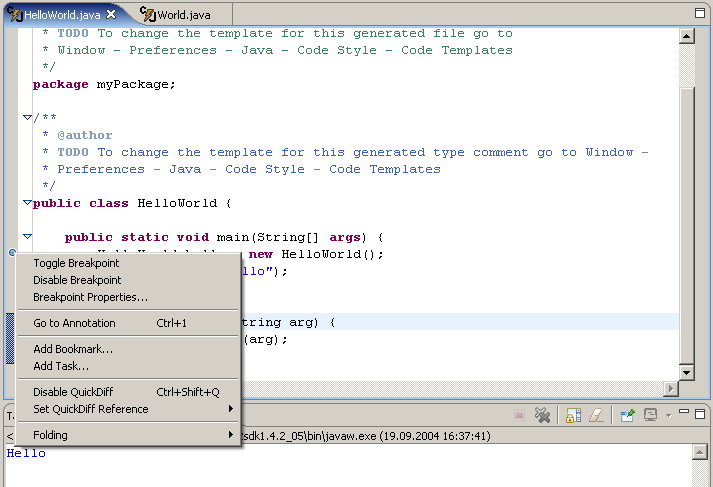
\includegraphics[width=0.60\textwidth]{images/brake_point.png}
	\caption{Toggling a debugging breakpoint}
	\label{fig:brake_point}
\end{figure*}

After setting one or more breakpoints, you launch the Eclipse debugger in the normal way by clicking on the debug icon in the toolbar. The debugger perspective looks like figure \ref{fig:debuger}.
\begin{figure*}[htbp]
	\centering
		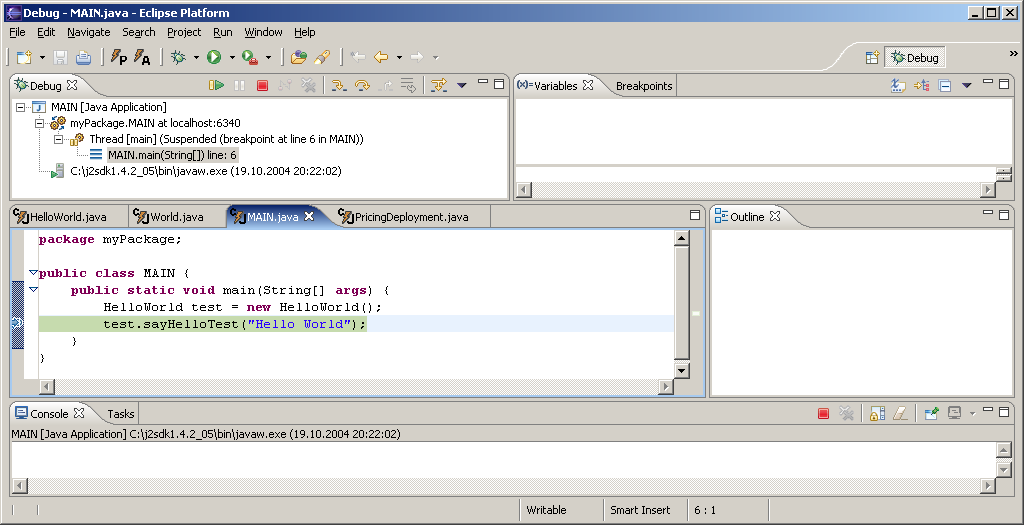
\includegraphics[width=1.0\textwidth]{images/debug1.png}
	\caption{Debugger perspective}
	\label{fig:debuger}
\end{figure*}

You can use the Java Debug step filters (\markedtext{Window} $\rightarrow$ \markedtext{Preferences} $\rightarrow$ \markedtext{Java} $\rightarrow$ \markedtext{Debug} $\rightarrow$ \markedtext{Step Filtering}) to make this process a little easier.\\
\textbf{Note:} A current limitation is that you cannot set breakpoints in cclasses.